\section{Study design}
\label{sec:sherloc-design}


% \label{sec:design}

% \begin{figure*}[ht]
% \centering
% 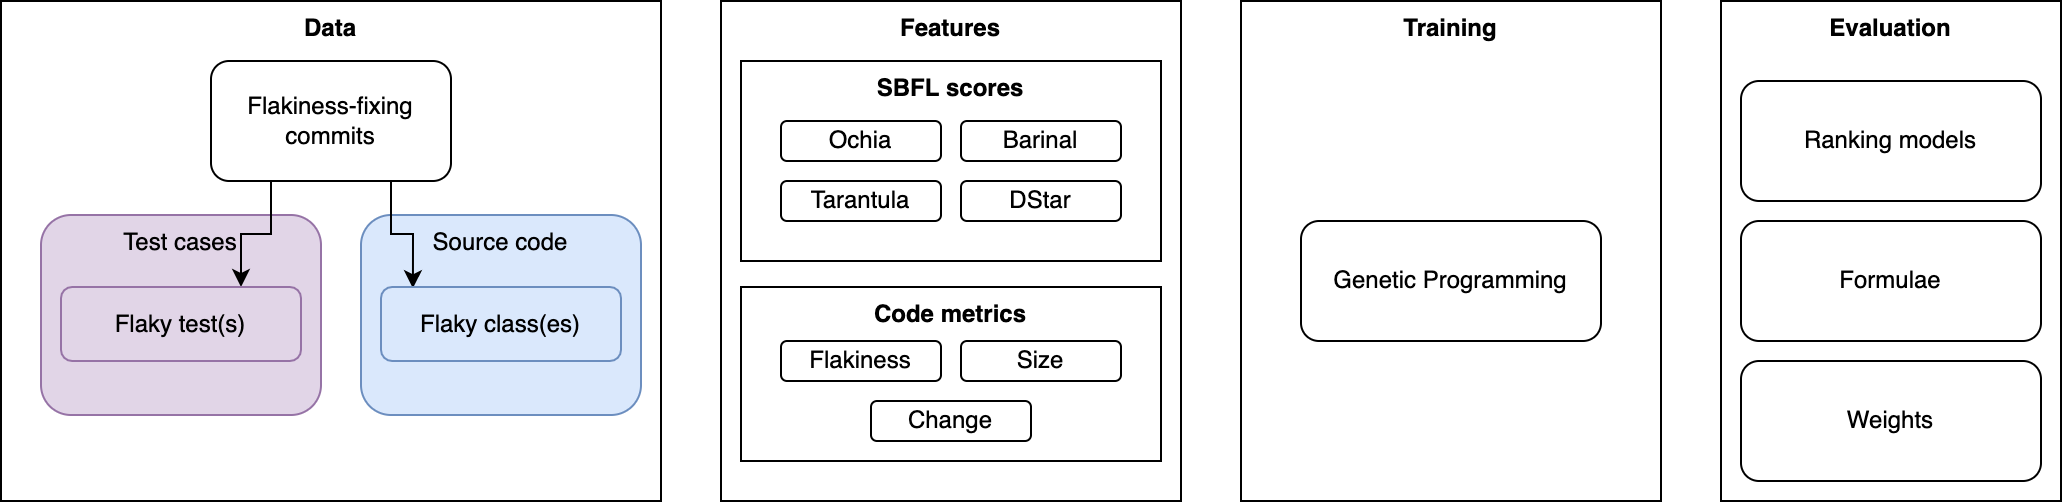
\includegraphics[width=0.7\linewidth]{figures/sherloc/design_summary.png}
% \caption{Summary of the study design.} 
% % \centering}
% \label{fig:study_design}
% \end{figure*}



%In this section, we explain for each research question: the motivation behind it and the approach followed to answer it. 



%Figure~\ref{fig:study_design} summarises the main steps of this process. 


%the data collection and extraction processes and present our data analysis approach for answering each research question.

\subsection{RQ1 - Effectiveness}\label{sub:rq1_effectiveness}
\subsubsection{Motivation}\label{subsub:rq1_motivation}
The objective of our study is to investigate the usability of well-founded FL techniques to help in mitigating flaky tests.
The literature on FL proposes a wide variety of categories such as ML-based techniques~\cite{Lou:2021:fse,Li:2019:issta,briand2007}, mutation-based techniques~\cite{Papadakis:2015sf,Hong:2015db}, and qualitative reasoning-based techniques~\cite{perez2018leveraging}.
% The literature on FL proposes a w
Nonetheless, spectrum-based fault localisation remains one of the most distinguished FL categories thanks to its effectiveness and simplicity~\cite{wong2016survey}. % the survey one
%its solid performances~\cite{??} and the considerable number of approaches building on it~\cite{??}.
SBFL requires only the test coverage matrix to compute the likelihood for a code entity to include the root cause of an observed test failure. 
The main assumption of SBFL is that code entities covered by more failing tests and fewer passing tests are more suspicious than those less covered by failing tests and more by passing tests~\cite{renieres2003fault}.
This assumption can be revised to identify the root causes of flaky tests instead of bugs.
In particular, if we separate tests into two groups: \textit{flaky} and \textit{stable}, instead of \textit{failing} and \textit{passing}, we can leverage the coverage matrix to rank classes based on their correlation with flaky tests. 
In this case, the assumption would be that classes covered by more flaky tests and fewer stable tests have a higher chance to be responsible for test flakiness.
In this RQ, we assess the effectiveness of this adaptation of SBFL in identifying flaky classes. 


\subsubsection{Approach}\label{subsub:rq1_approach}
Relying on the data collected in Section~\ref{sec:sherloc-data}, we use the \textsc{GZoltar} plugin to run the test suites of each commit and build coverage matrices.
Based on these matrices, we compute for each class the spectrum data: $(e_{s}, e_{f} , n_{s}, n_{f})$.
In our case, for each class, $e_{s}$ and $e_{f}$ represent the number of stable and flaky tests executing it, respectively.
On the other hand, $n_{s}$ and $n_{f}$ represent the number of stable and flaky tests that do not execute it, respectively.
To compute classes' suspiciousness scores, we inject these spectrum data in classical SBFL formulæ.
Table~\ref{tab:formulae} summarises the four formulæ adopted in our study with the necessary adaptations for flakiness.
For DStar, the notation ‘*’ is a variable that we set to 2 based on the recommendation of Wong \etal~\cite{wong-dstar}.
With each formula, we compute the suspiciousness scores of each class and then rank them in descending order: classes with the highest scores are ranked first.

%To assess the effectiveness of SBFL, we contrast the ranking of the actual culprit class by each formula with the actual 
Recently, it has been  theoretically proven that no SBFL formula can outperform all others~\cite{Yoo:2014fv}. In addition, Xuan and Monperrus proposed a new approach that learns to combine multiple SBFL \formulas~\cite{monperrus-ICSME}. Their approach, called Multric, successfully outperformed all the input \formulas, opening a trend to use multiple \formulas to overcome the limitation of using a single SBFL formula~\cite{B.-Le:2016yu,zou2019empirical,Li:2019:issta}. 
Following this trend, we used Genetic Programming to evolve a new formula that combines all four SBFL \formulas. 

%Besides the ranking provided by our formulae, we evolve new formula using genetic programming.
%GP is an evolutionary algorithm that leverages mutation, crossover, and a fitness function to evolve a fit program.
%In our case, we use GP to evolve a ranking model that takes as input the suspiciousness scores provided by the \formulas and outputs a ranking. Our fitness function for GP evaluates the models based on their average ranking of flaky classes.
%For crossover and mutation, we use a single-point crossover with a rate of 0.9 and subtree mutation with a rate of 0.1. We configure the GP to have a population of 40 individuals and to stop after 100 generations. Each individual of the population denotes a single candidate formula and is generated using six arithmetic operators (i.e., subtraction, addition, multiplication, division, square root, and negation), a constant one, and the features that GP takes as input.
% here, explain all the details ..? and reference them for rq2..?
%We use ten-fold cross-validation to maximise our data usage and prevent our model from overfitting to the training data. We also normalise all our input data between 0 and 1 using min-max normalisation. 
%To compensate for the inherently stochastic nature of GP, we run GP 30 times with 30 different random seeds and report the results of a model with the median fitness. For the implementation of GP, we use DEAP v.1.3.1~\cite{Fortin:2012aa}. 
Genetic Programming (GP) evolves a solution (\ie a program) for a given problem under the guidance of a (fitness) function. %As GP represents each solution as a tree, it is often used as a symbolic regression tool. Another noteworthy feature of
GP can also  generate non-linear models and learn a model flexibly from input instead of defining a fixed formula. Hence, GP was employed to generate risk evaluation \formulas for fault localisation~\cite{Yoo:2017ss,sohn-TSE}. 
For the same reasons, we employ GP to evolve a model (\ie a formula) for the flaky class identification problem. 
We configure the GP to have a population of 40 individuals and to stop and return the best model found so far after 100 generations. 
Each individual in the population denotes a single candidate formula and is generated using (i) six arithmetic operators (subtraction, addition, multiplication, division, square root, and negation) and (ii) the features that GP takes as input.
We define our fitness function as the average ranking of flaky classes. To make most of the data and avoid overfitting, we use ten-fold cross-validation, using one fold for test and the others for training. We also normalise all input data between 0 and 1 using min-max normalisation. 
Finally, to compensate for the inherently stochastic nature of GP, we run GP 30 times with different random seeds and report the results of a model with the median fitness. %For the implementation of GP, w
We used DEAP v.1.3.1~\cite{Fortin:2012aa}. 

\begin{table}
\vspace{-0.5em}
\centering
\caption{SBFL formulae adapted to flakiness.
\vspace{-0.5em}
%\\
% $e_f$: number of flaky tests executing the class.\\
% $e_s$: number of stable tests executing the class.\\
% $n_f$: number of flaky tests not executing the class.\\
% $n_s$: number of stable tests not executing the class.
\centering}
\label{tab:formulae}
%\resizebox{\columnwidth}{!}{
\begin{tabular}{lc} 
\toprule
 \textbf{{Name}} & \textbf{{
Formula}}   \\  \hline
Ochiai~\cite{Abreu:2006yf} & $\frac{e_f}{\sqrt{(e_f + n_f)(e_f + e_s)}}$ \\ %\hline
Barinel~\cite{abreu2009spectrum} & $1 - \frac{e_s}{e_s + e_f}$ \\ %\hline
Tarantula~\cite{Jones:2001vn,Jones:2002kx} & $\frac{\frac{e_f}{e_f+n_f}}{\frac{e_f}{e_f+n_f}+\frac{e_s}{e_s+n_s}}$ \\ %\hline
DStar~\cite{wong-dstar} & $\frac{e_f^*}{e_s * n_f}$ \\\bottomrule
\end{tabular}
%}
\vspace{-6mm}
\end{table}
%\paragraph{Evaluation:}
\subsection{RQ2 - Code and change metrics}
\subsubsection{Motivation}
The objective of this question is to explore the benefits of augmenting the SBFL technique with additional signals from the software.
Recent studies showed that the performances of SBFL can be improved by incorporating signals from code and change metrics.
More specifically, Sohn and Yoo~\cite{sohn-TSE} showed that combining SBFL with code and change metrics widely adopted in the fault prediction community~\cite{McI:2018:tse}, such as age, change frequency (\ie churn), and size, can significantly improve the approach's performances.
%These metrics used by Sohn and Yoo~\cite{sohn-TSE} are widely adopted by the defect prediction community~\cite{McI:2018:tse,Kamei:2012:tse}, as they provide guidance about faulty code entities.
The assumption is that code entities with higher complexity and change frequency are more likely to be faulty.
Several studies suggested that the test size and complexity can also be an indicator of flakiness~\cite{Pinto2020,King2018,Camara2021a}. % 
However, it is unclear if such metrics correlate also with classes that are responsible for test flakiness.
Therefore, in this RQ, we assess the benefits of these metrics in spotting flaky classes.
Besides these metrics, we investigate the effects of metrics that are specific to the nature of flaky tests.
Multiple empirical studies analysed the root causes of flakiness and showed that the main categories are: Async Waits, Concurrency, Order-dependency, Network, Time, I/O operations, Unordered collections and Randomness~\cite{Luo2014,Parry2021,Lam2020a,Gruber2021}.
We derived a list of static metrics that describe each of these categories in Java projects.
We exclude order-dependency because order-dependent tests generally stem from tests themselves instead of the CUT, thus, they are not concerned by our approach.
In the following, we describe our approach for (i) calculating these metrics and (ii) defining a FL formulae based on them.
%This RQ aims to assess the effectiveness of similar change and code metrics in the pinpointing the roots of flakiness.

%Despite its good performances, several studies highlighted the limits of SBFL~\cite{??}
\subsubsection{Approach}

\paragraph{Metric collection}
Table~\ref{tab:metrics} summarises the full list of metrics used in our study.
To compute these metrics, we first retrieve the source code of the project at the commit of interest (\ie the parent commit of the flakiness-fixing commit identified by the data collection step).
Then, for calculating flakiness-specific metrics, we use Spoon~\cite{spoon}.
Spoon is a framework for Java-based program analysis and transformation that allows us to build an abstract syntax tree and a call graph.
Using the graph and tree, we extract classes and their metrics (\eg \#COPS and \#ROPS). 
For size metrics, we also use these code analysis results from Spoon (\eg DOI). 
As for change metrics, we analyse the change history and extract the following information: the date of each commit, files modified and renamed by each commit, and authors of individual commits. Using this information, we compute the three change metrics: Unique Changes, Age, and Developers.

%\renewcommand{\arraystretch}{1}
\begin{table}
\vspace{-0.5em}
\begin{center}
\caption{Code and change metrics used to augment SBFL.\centering}
\vspace{-0.5em}
\label{tab:metrics}
%\resizebox{\columnwidth}{!}{
\begin{tabularx}{\columnwidth}{l|l|X} 
\cmidrule[\heavyrulewidth]{2-3}
\textbf{{}} & \textbf{{Metric}} & \textbf{{Definition}} \\ \midrule
\multirow{10}{*}{\rotatebox[origin=c]{90}{Flakiness}} & \#TOPS & Number of time operations performed by the class.\\ \cline{2-3}
& \#ROPS & Number of calls to the \texttt{random()} method in the class.\\ \cline{2-3}
& \#IOPS & Number of input/output operations performed by the class.\\ \cline{2-3}
& \#UOPS & Number of operations performed on unordered collections by the class.\\ \cline{2-3}
& \#AOPS & Number of asynchronous waits in the class.\\ \cline{2-3}
& \#COPS & Number of concurrent calls in the class.\\ \cline{2-3}
& \#NOPS & Number of network calls in the class. \\
\midrule 

\multirow{3}{*}{\rotatebox[origin=c]{90}{Change}} & Changes & %The ratio between the number of commits modifying the code class and the total number of commits in the repository
Number of unique changes made on the class. \\ \cline{2-3}
& Age & %The distance between the commit that introduced the code entity and the current one. 
Time interval to the last changes made on the class. \\ \cline{2-3}
& Developers & Number of developers contributing to the class. \\ \midrule

\multirow{3}{*}{\rotatebox[origin=c]{90}{Size}} & LOC & The number of lines of code.\\ \cline{2-3}
& CC & Cyclomatic complexity.\\ \cline{2-3}
& DOI & Depth of inheritance.\\ 
\bottomrule
\end{tabularx}
%}
\end{center}
\vspace{-4mm}
\end{table}

%JJ: TO-DO 
\paragraph{Ranking model}
Similarly to RQ1, we use GP in order to generate models that combine our metrics with suspiciousness scores generated by SBFL \formulas.
In particular, for each type of metrics (\ie flakiness, size, and change), we evolve a model that takes as input its metrics with SBFL scores and outputs a ranking for each candidate class.
Afterwards, we compare the performances of these models to infer the contribution of each type of metrics.



\subsection{RQ3 - Ensemble method}\label{sec:rq3_ensemble_method}
\subsubsection{Motivation}
This question explores the potential for improvement by exploiting all the \formulas generated using GP while at the same time making the most of the resources spent on model generation.
% If we can show ...... => chgs, age, size .... 
For this aim, we use voting as our ensemble learning method.
We opted for voting since it does not require an additional cost for model generation and its effectiveness has already been demonstrated by previous fault localisation studies~\cite{Sohn2021ea,Sohn2019aa}

\subsubsection{Approach}
%Voting between models goes through two phases: candidate selection and voting. During the candidate selection phase, all models participating in the voting compute the score for each candidate. A candidate in our case is an individual class of the CUT. In the voting phase, we sort the candidates in a descending order based on their scores.Then, the models vote for candidates placed within the top $N$. We aggregate these votes and reorder the voted candidates from the most voted to the least voted. 
Voting between models is performed in two phases: candidate selection and voting. During the candidate selection phase, all the participating models compute their own suspciousness scores for the candidates. A candidate, in our case, is an individual class of the CUT. %Candidates are sorted in descending order based on their scores, and those placed within the top $N$ are selected as the final voting candidates. 
Individual models compute their own suspiciousness scores for the candidates and select those placed within the top $N$ as their candidates to vote.
In the voting phase, each model votes for its own top $N$ candidates. If $M$ number of models participate in the voting, we can have the maximum $N \times M$ number of voted candidates in total. The votes from the models are then aggregated, and the voted candidates are reordered from the most voted to the least voted. 


Previous studies on voting-based FL showed that varying the number of votes that each candidate receives based on its actual rank in individual models can improve the localisation performance even further~\cite{Sohn2021ea,Sohn2019aa}.
Hence, rather than assigning the same number of votes to each candidate, we allow individual models to cast a different number of votes for each candidate based on its location in the ranking. 
For instance, a candidate ranked at the top will obtain a complete one vote, whereas a candidate ranked in the third place will get $\frac{1}{3}$ vote. 
As mentioned in~\ref{Tie-breaking}, candidates can be tied with other candidates since their ranks are computed from ordinal scores. When a candidate fails to be in the top $N$ due to being tied with others, we allow every tied candidate ($c$) to receive the following number of votes:
$votes = \frac{1}{rank_{best}(c) \times n_{tied}(c)}$ votes. 
%\[ votes = \frac{1}{rank_{best} \times n_{tied}}\]  
Here $rank_{best}$ denotes the best (highest) rank a tied candidate can have, and $n_{tied}$ is the total number of tied candidates, including itself. The equation below summarises the number of votes a candidate ($c$) can obtain. $rank(c)$ is the rank of the candidate $c$. 

\vspace{-4mm}
\[
\left\{ 
  \begin{array}{ c l }
    \frac{1}{rank(c)} & \quad \textrm{if } rank(c) \leq N \\
    \frac{1}{rank_{best}(c) \times n_{tied}(c)} & \quad \textrm{if } rank_{best}(c) \leq N \\
    0                 & \quad \textrm{otherwise}
  \end{array}
\right.
\]

\subsection{RQ4 - Flakiness categories}
\subsubsection{Motivation}
The literature on flaky tests reports different categories of flakiness~\cite{Luo2014,Parry2021,Lam2020a,Gruber2021}.
These categories can manifest differently both in the test and CUT and as a result the identification of flaky classes can also be affected by such differences.
That is, a technique might identify decently the classes responsible for non-deterministic network operation, but struggles in pinpointing classes causing race conditions.
%This RQ aims to evaluate the performances of SBFL-based models on distinct flakiness categories.
This RQ aims to investigate the performances of an SBFL-based approach among distinct flakiness categories.

\subsubsection{Approach}
Many studies manually analysed flakiness-fixing commits to categorise them~\cite{Luo2014,Thorve2018} based on their commit message and code changes.
In our study, we followed a similar process where two authors manually analysed the commits separately to assign them to one of the categories derived by Luo~\etal~\cite{Luo2014}.
As our manual analysis does not intend to build a new taxonomy or identify new categories, it is reasonable to adopt an existing taxonomy as reference.
The two authors had a disagreement over one commit, where one author only suggested one category whereas the other suggested two categories.
After discussion, the authors decided to keep two categories to avoid discarding relevant information.
The results of this analysis are available in our replication package.
After labelling the flakiness-fixing commits, we analyse the performance of our SBFL-based approach among different flakiness categories. 


\subsection{Evaluation metrics}
For the evaluation of our approach, we use two metrics: accuracy and wasted effort. 
Both \textit{acc@n} and \textit{wef} are based on the absolute number of code entities instead of percentages.
This conforms to the recommendations of Parnin and Orso~\cite{parnin} who suggested that absolute metrics reflect the actual amount of efforts required from developers better than percentages. 
The accuracy (\textit{acc@n}) calculates the number of cases where the flaky classes were ranked in the top $n$.
In our study, we report the \textit{acc@n} with 1, 3, 5, and 10 as n values. % cite 
In the cases of multiple flaky classes, we consider the flaky class to be among the top $n$, if at least one of the flaky classes is.
The second metric, wasted effort (\textit{wef}), allows us to measure the effort wasted while searching for the flaky class. It is formally defined as~\cite{monperrus-ICSME}:
\[ wef = |{susp(x) > susp(x*)}| + |{susp(x) = susp(x*)}|/2 + 1/2\]
Where $susp()$ provides the suspiciousness score of the class $x$, $x*$ is the flaky class, and $|.|$ provides the number of elements in the set. Accordingly, \textit{wef} measures the absolute number of classes inspected before reaching the real flaky class $x*$. 
%As wef only gives the absolute number of classes investigated before finding the flaky class, we wanted to balance this information with regards to the total number of classes covered by flaky tests. Accordingly, we also report, enclosed in parentheses in table VII, the average of wasted effort out of the total number of classes covered by flaky tests

For our approach to be useful for developers, it should provide guidance beyond currently available information. 
%When a program fails due to flaky tests, the first thing developers can do to locate the source of flakiness is to inspect the code entities covered by the flaky tests. 
When a program fails due to flaky tests, one thing that can be helpful to identify the cause is a list of classes covered by the flaky tests.
Hence, in this paper, we count the total number of classes covered by flaky tests (\ie our baseline) and compare it with the number of classes inspected to locate a flaky class (\ie \textit{wef}$+1$). 
More specifically, in addition to the two absolute metrics, we measure the relative effort defined as:
\[R_{wef} = \frac{100 \times (wef + 1)}{\text{\# of classes covered by flaky tests}}\text{, } 0 < R_{wef} \leq 100\]
%$R_{wef} = \frac{wef + 1}{\text{\# of classes covered by flaky tests}}$

If $R_{wef}$ is smaller than 50, we consider our approach to outperform the baseline since it saves more than the expected effort (\ie average) of the baseline.

\subsection{Tie-breaking}
\label{Tie-breaking}
Both SBFL and our evolved \formulas compute an ordinal score for each class. As a result, multiple classes can have the same score, being tied to each other. Ties are generally harmful as they force developers to inspect more classes. Among various tie-breakers introduced and adopted to handle this problem~\cite{xu2011ties}, we use a max tie-breaker that assigns the lowest rank (\ie the maximum) to all tied entities. We choose the max tie-breaker to avoid overinterpretation of the results. 